\subsection{DAC Power Amp} \label{subsec:DAC_Filter}
The system is to test impedance over a broad range of \SIQ{100}{\milli\ohm} to \SIQ{100}{\mega\ohm}, according to requirement §3 from section \ref{ch:SystemRequirements}. In order to excite impedances, especially in the range of \SIQ{10}{\ohm} and lower, a power amplifier is required. This amplifier must be capable of driving both reactive and passive devices. This is achieved by the use of controlled output impedance and the utilized range resistors used to measure the DUT current. 

The amplifier is designed as a class AB amplifier output stage and a high speed op-amp. The circuit used can be seen in figure \ref{fig_7_1_1_5_DAC_POWER_AMP}.

\begin{figure}[H]
    \centering
    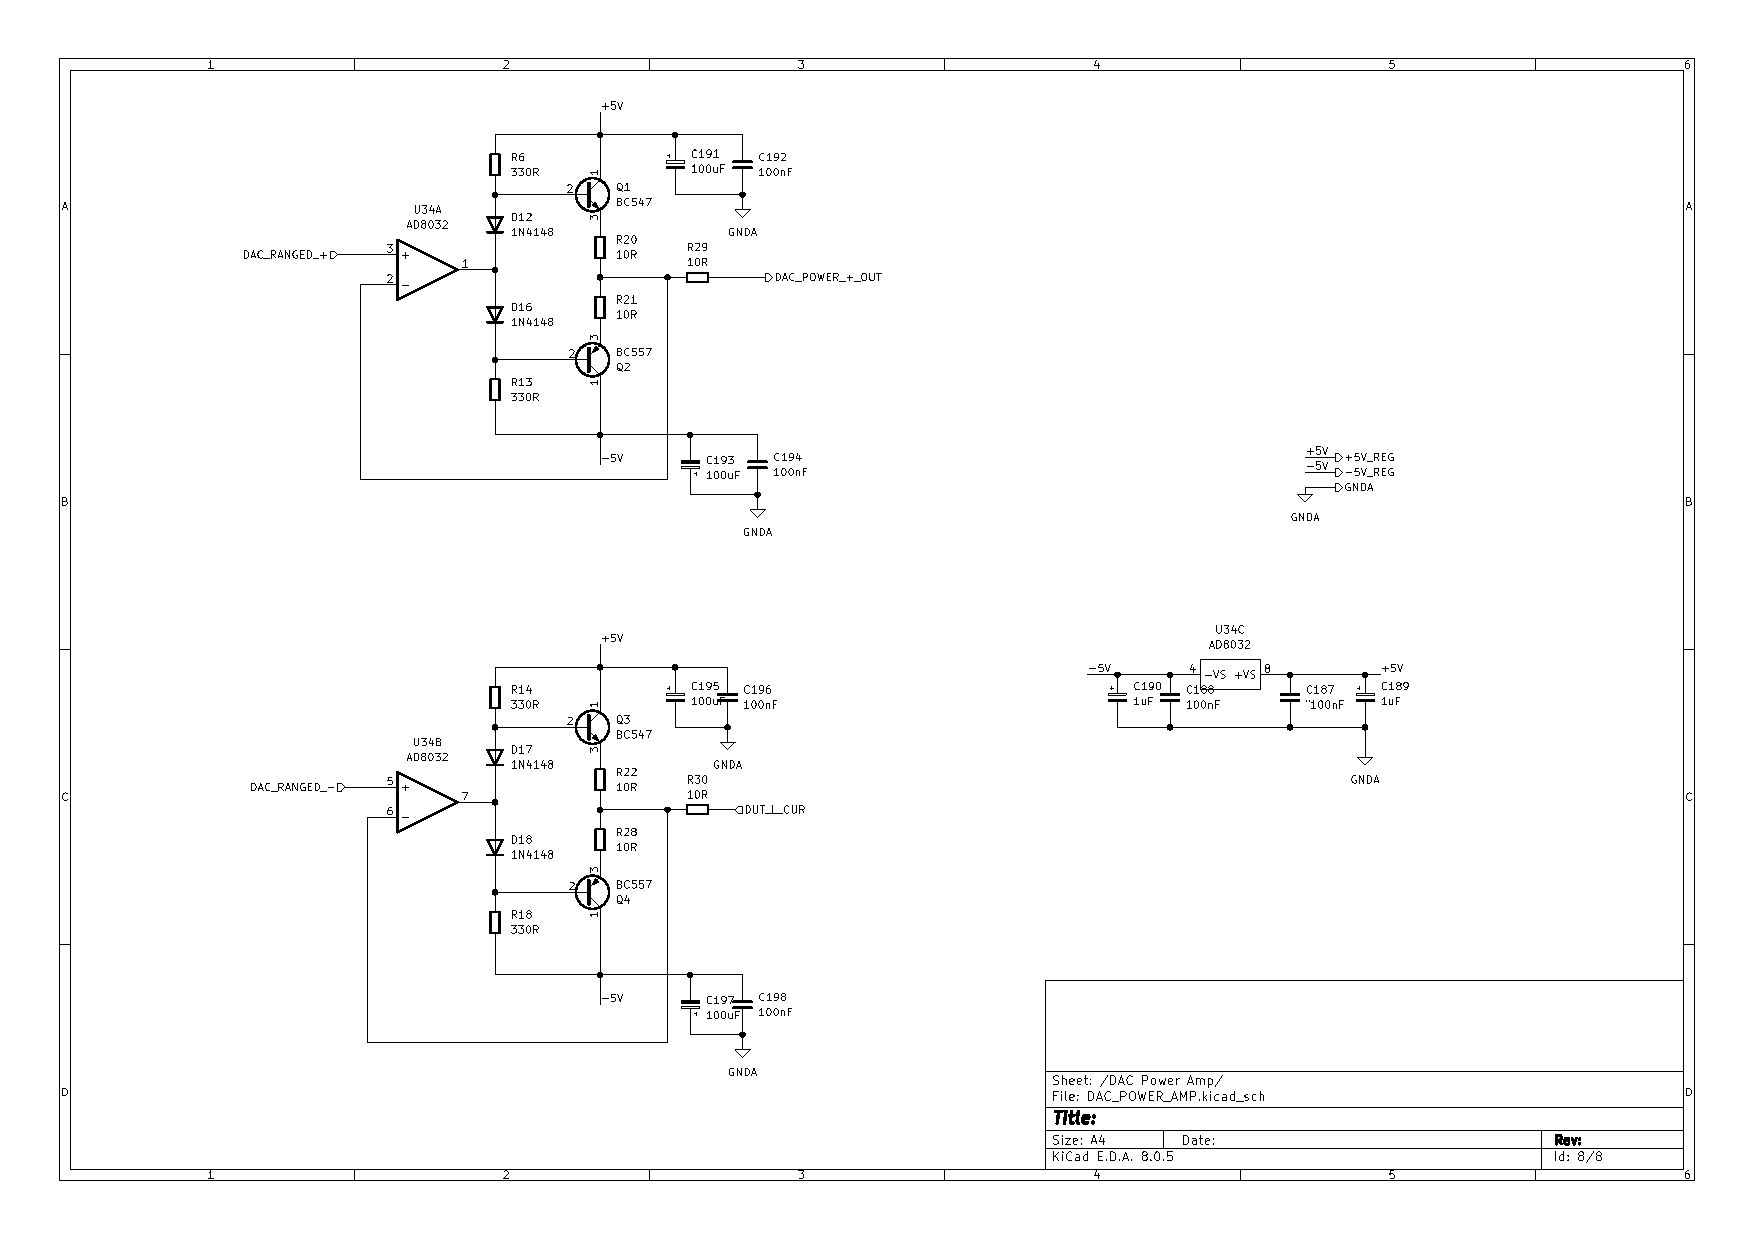
\includegraphics[clip, trim=150 320 415 40, width=0.9\textwidth]{Sections/7_SystemDesign/Figures/7_1_1_5_DAC Power Amp.pdf}
    \caption{DAC power amplifier circuit, positive side of the differential output.}
    \label{fig_7_1_1_5_DAC_POWER_AMP}
\end{figure}

About \SIQ{15}{\milli\ampere} of bias current for the output stage has been chosen. From BC547B and BC557 datasheets, \cite{BC547_datasheet} \cite{BC557_datasheet}, the base-emitter voltage can be found to be roughly \SIQ{730}{\milli\volt} at a collector current of \SIQ{15}{\milli\ampere}. This bias-current is set by the use of a simply diode. This adds some thermal stability, given they are thermally closely linked, as the temperature coefficient of a diode is negative, whilst positive for a transistor. The required DC current for a 1n4148 diode to have a voltage-drop of \SIQ{730}{\milli\volt} is estimated to \SIQ{12}{\mA}. The supply voltage is from a split supply of $\pm$ \SIQ{5}{\volt}, resulting in a total supply voltage of \SIQ{10}{\volt}. Assuming that the two biasing diodes, D12 and D16 in figure \ref{fig_7_1_1_5_DAC_POWER_AMP}, are matched the voltage across the biasing resistors R6 and R13 will be $10-2\cdot0.73 = $\SIQ{8.54}{\volt}. Combined series resistance of R6 and R13 can be estimated as $\frac{8.54 V}{0.012 A} = $ \SIQ{712}{\ohm}. Resistors of \SIQ{330}{\ohm} has been chosen, producing a biasing current of \SIQ{12.9}{\milli\ampere}.

To increase the input impedance and reduce output distortion of the amplifier, an op-amp is used with the output class AB stage in its feedback loop. The used op-amp is an \SIQ{80}{\mega\hertz} GBW op-amp, AD8032 \cite{AD8032_datasheet}. 

\subsubsection{Stability}
Driving reactive, especially capacitive loads can pose a challenge to any feedback system with a phase margin less than \SIQ{90}{\degree}. The typical phase-margin of an op-amp is in the range of \SIQ{45}{\degree}, leading to potential instability when driving capacitive loads.

A way to counteract the risk of instability, is to introduce a zero in the transfer function of the feedback path by inserting a series resistance with the output of the feedback system, this is also known as an isolation resistor. This resistor should be placed outside of the feedback loop, the value of this resistor will depend upon the load capacitor. This indicates that a stability analysis of the DAC power amp should be conducted, as it is very likely that a user would load the system with a capacitive load. This analysis is based on the block diagram of the differential DAC output, depicted in figure \ref{fig_7_1_1_5_DAC_POWER_AMP_BLOCK}. 


\begin{figure}[H]
    \centering
    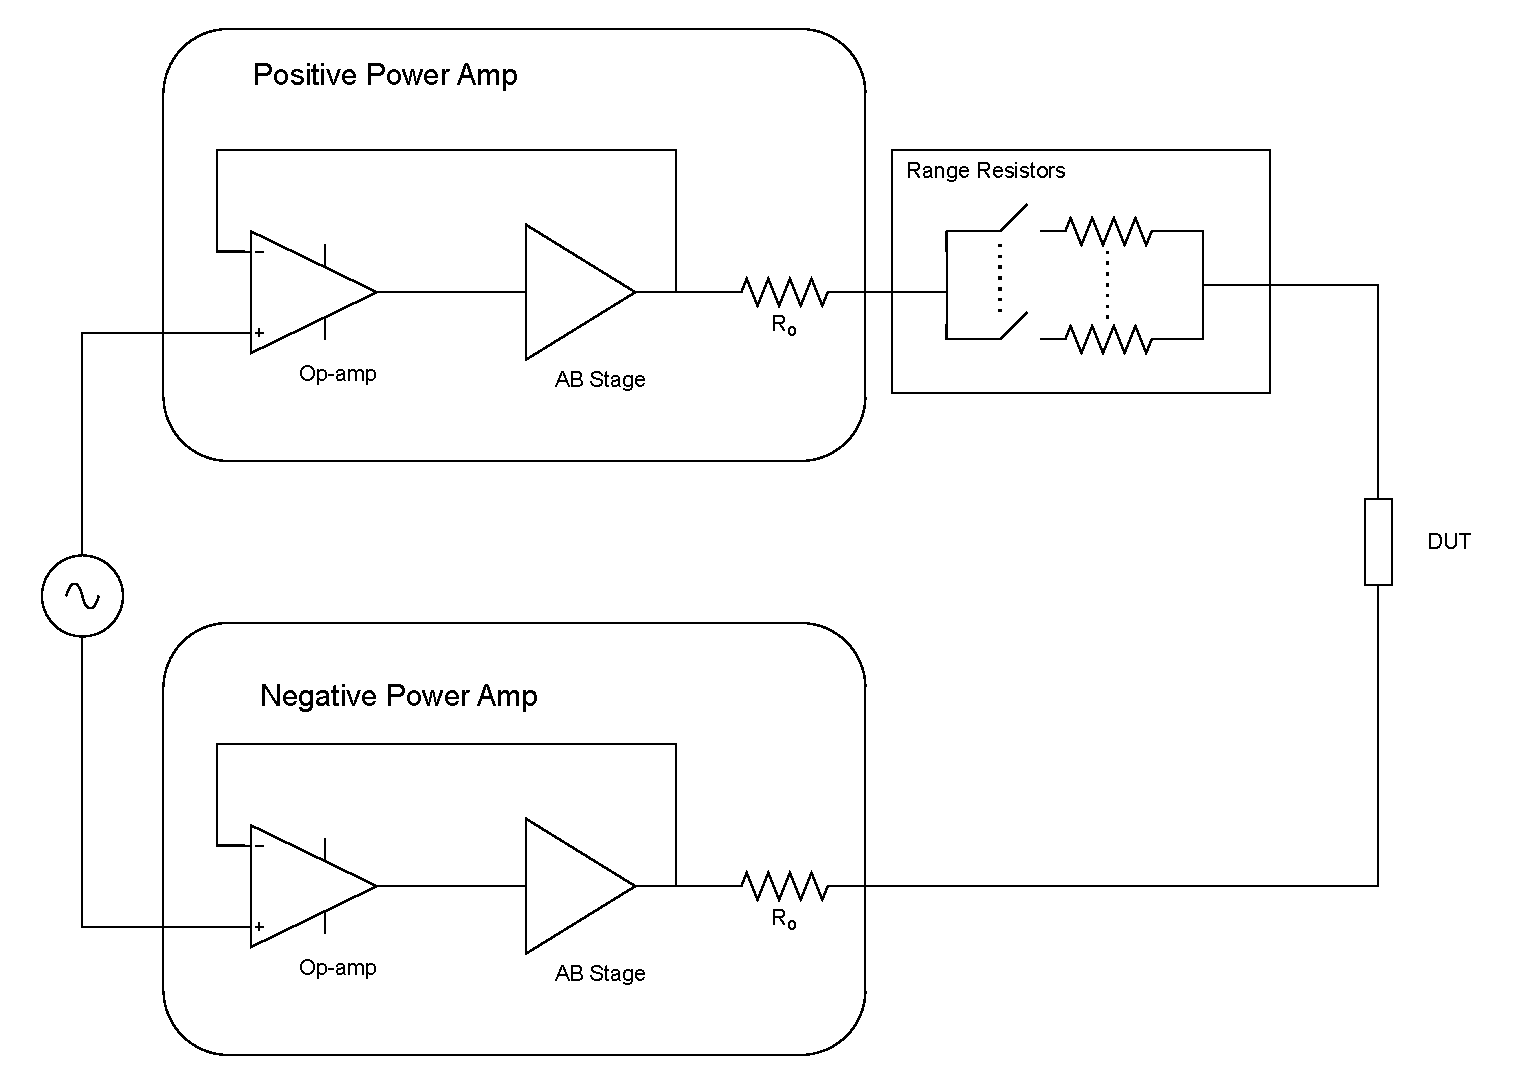
\includegraphics[clip, trim=0 0 0 0, width=0.9\textwidth]{Sections/7_SystemDesign/Figures/DAC_POWER_BLOCK.pdf}
    \caption{Block diagram of the differential DAC power amp output stage.}
    \label{fig_7_1_1_5_DAC_POWER_AMP_BLOCK}
\end{figure}

The stability analysis is simplified by only looking at the positive side of the differential output seen in figure \ref{fig_7_1_1_5_DAC_POWER_AMP_BLOCK}. Here $R_o$ is then replaced by $2\cdot R_o$. One thing to take note of here, is that the range resistors can be used both as current shunts and isolation resistors. The stability analysis aims to ensure that when the output is capacitively loaded, the appropriate range resistor will establish stability.

To analyze the output stage, the op-amp is modelled as a two pole \SIQ{80}{\mega\hertz} GBW, \SIQ{30}{\degree} phase margin op-amp with \SIQ{80}{\decibel} open-loop DC gain, based on the datasheet information of the used AD8032 \cite{AD8032_datasheet}. The class AB output stage is modelled as a small signal emitter follower. Using a small signal model might seem somewhat unsuitable for the output stage, as it does not operate with small signals. The small signal model has however proved to produce approximately accurate bandwidth information, even for large signals.

The simplified small signal model is derived from the diagram shown in figure \refq{fig_7_1_1_5_DAC_POWER_AMP_ss}

\begin{figure}[H]
    \centering
    \includegraphics[clip, trim=80 150 100 50, width=1\textwidth]{Sections/7_SystemDesign/Figures/DAC_POWER_ss.pdf}
    \caption{Small signal model of the differential output power stage.}
    \label{fig_7_1_1_5_DAC_POWER_AMP_ss}
\end{figure}

Simulation has been used for the stability analysis. LTspice from Analog Devices is capable of directly simulating the circuit shown in figure \refq{fig_7_1_1_5_DAC_POWER_AMP_ss}, as well as simulating the behaviour of a two pole op-amp. The simulated model can be seen in figure \refq{fig_7_1_1_5_DAC_POWER_AMP_SIM}, here UniversalOpAmp3 is a programable op-amp that has been set to an open-loop DC gain of \SIQ{80}{\decibel}, GBW of \SIQ{80}{\mega\hertz} and a phase margin of \SIQ{30}{\degree}. The specific transistor parameters, $r_x, r_\pi, c_\pi$ and $c_\mu$ have been derived from the datasheet of a BC557B and experiance with the specific transistor. The PNP and NPN transistors of the push-pull output have been estimated as being only PNP transistors, as PNP semiconductors are of worse performance than their NPN counterparts. 

\begin{figure}[H]
    \centering
    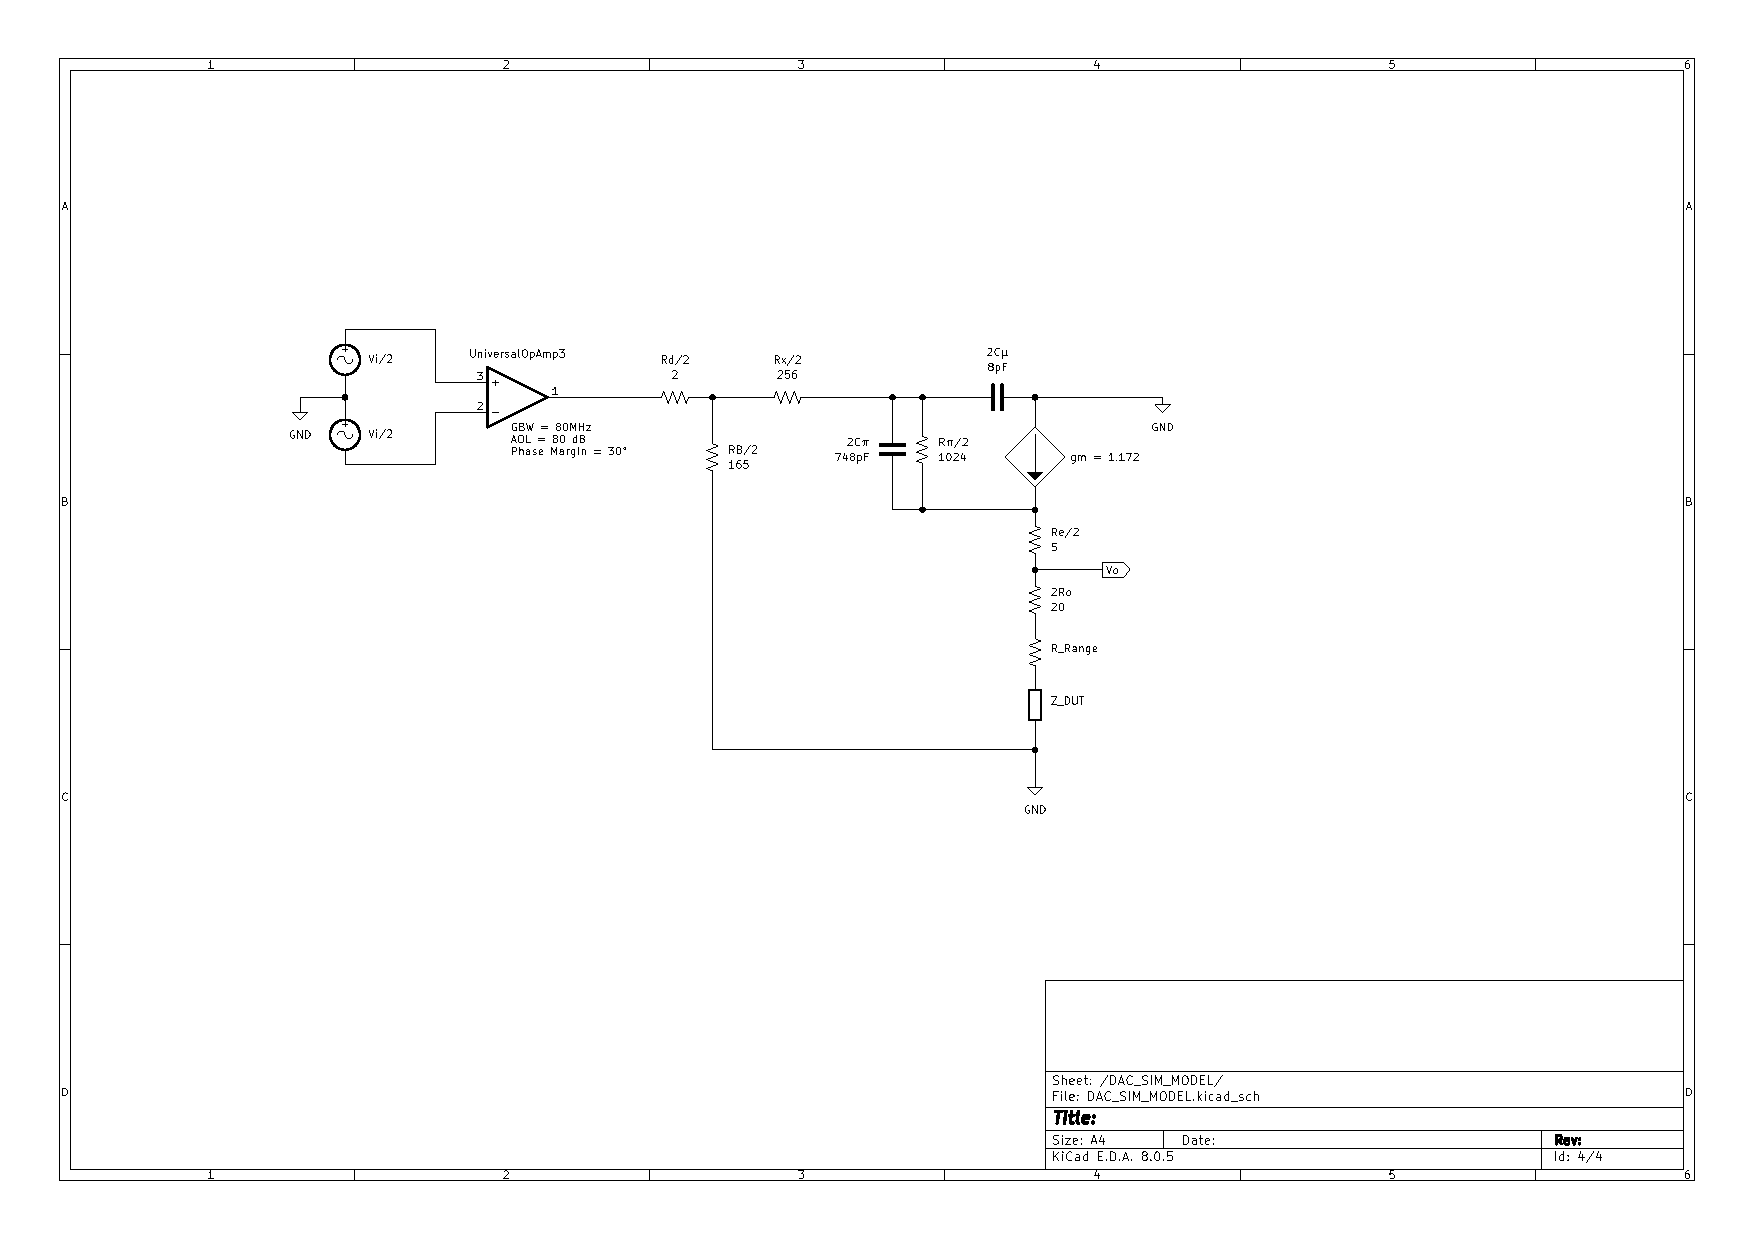
\includegraphics[clip, trim=130 200 220 150, width=1\textwidth]{Sections/7_SystemDesign/Figures/7_1_1_5_DAC_FILTER-DAC_SIM_MODEL.pdf}
    \caption{The simulated model for the DAC power amp, simulated using LTspice from Analog Devices. Notice that the op-amp is in an open loop configuration, as stability analysis is performed.}
    \label{fig_7_1_1_5_DAC_POWER_AMP_SIM}
\end{figure}

The typical small signal gain of a BC557B can be approximated as the DC current gain, such that $H_{FE} \approx h_{fe}$. The datasheet of the BC557B \cite{BC557_datasheet}, indicates that the DC current gain at \SIQ{25}{\degreeCelsius} and \SIQ{15}{\milli\ampere} collector current is 300. The base collector capacitance $C_\mu$ can be directly found in the datasheet as $C_{ob}$, at a collector base voltage of \SIQ{-4}{\volt} the capacitance is \SIQ{4}{\pico\farad}. 

The transconductance gm is calculated by the use of the thermal voltage, and DC collector current. The thermal voltage is estimated to be \SIQ{25.6}{\milli\volt} at \SIQ{24}{\degreeCelsius}, the DC collector current is \SIQ{15}{\milli\ampere}, $gm = \frac{I_C}{V_T} = \frac{0.015}{0.0256} = 0.5859$. $r_\pi$ is estimated by the use of the current gain and transconductance as $r_\pi = \frac{h_{fe}}{gm} = \frac{300}{0.5859} = \SIQ{512}{\ohm}$. 

In order to find $r_x$, the black-box parameter $h[ie]$ is required. This parameter is not know, however experiance indicates that $r_x$ can be estimated as \SIQ{20}{\%} the value of $r_\pi$, and $r_x$ has been estimated as $r_x = \SIQ{102}{\ohm}$.

$C_\pi$ is estimated from the current gain bandwidth product of the transistor, found to be $f_t = \SIQ{245}{\mega\hertz}$ at a collector current of \SIQ{15}{\milli\ampere}. $C_\pi$ is then estimated as $C_\pi +C_\mu = \frac{gm}{2\cdot\pi\cdot f_t}$. This expression estimates the sum of $C_\pi$ and $C_\mu$, $C_\mu$ is however know and can simply be subtracted. $C_\pi = \frac{0.5859}{2\cdot\pi\cdot 245 MHz} -4 pF = 377 pF$. The small signal diode resistance $r_d$ is calculated as $r_d = \frac{V_T}{I_D}$, with an estimated temperature of \SIQ{24}{\degreeCelsius} and a diode DC current of \SIQ{12}{\milli\ampere}, the resistance is $r_d = \frac{0.0256}{0.012} \approx \SIQ{2}{\ohm}$. 

Note however that these are the estimated values for a single transistor in the push-pull output. The power amplifier has however been simplified in such a way that all these resistors and capacitors are in parallel, resulting in the capacitors doubling in value and resistors halfing.

\begin{figure}[H]
    \centering
    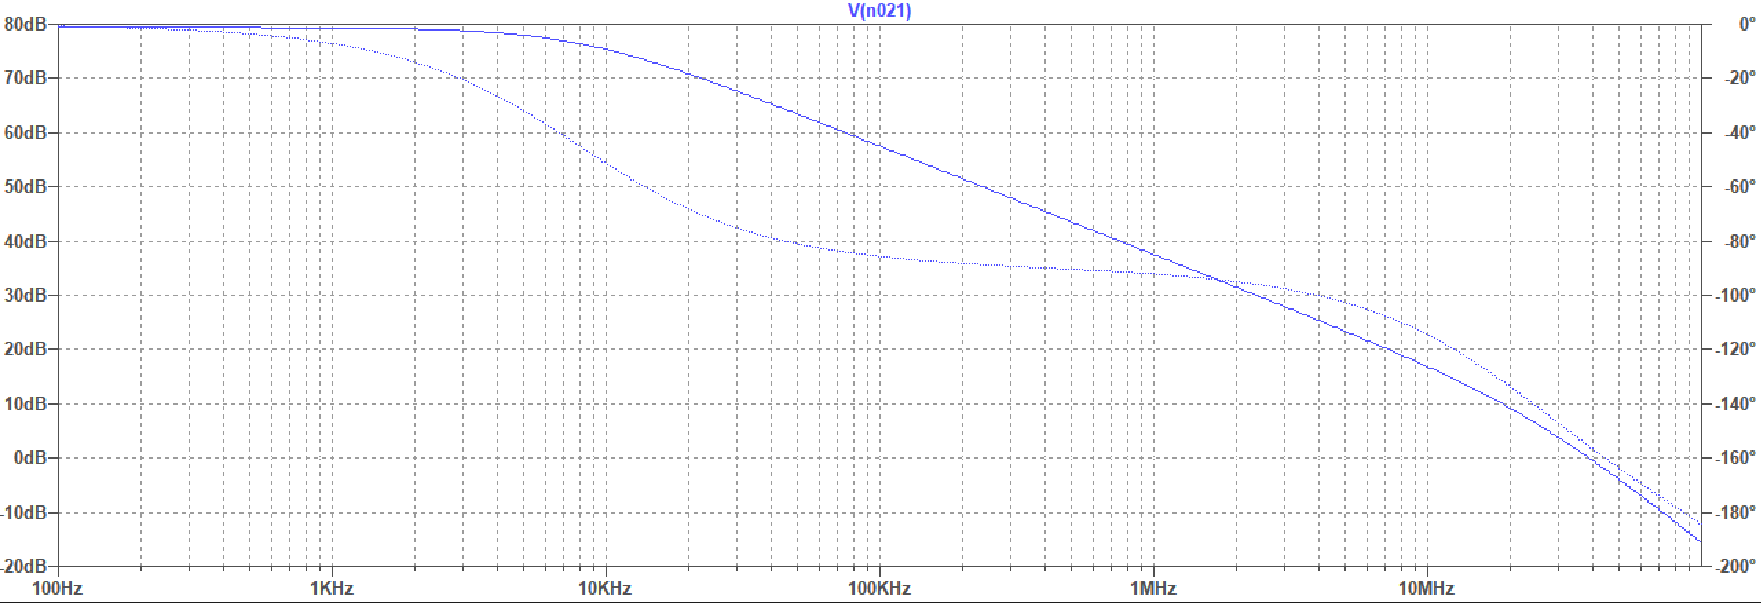
\includegraphics[clip, trim=0 0 0 0, width=1\textwidth]{Sections/7_SystemDesign/Figures/7_1_1_5_DAC_PWR_AMP_NO_LOAD.pdf}
    \caption{The simulated open-loop response of the DAC power amplifier with no load and a range resistor of \SIQ{1}{\ohm}.}
    \label{fig_7_1_1_5_DAC_POWER_AMP_SIM_NL}
\end{figure}


To analyze the system with no laod, an open-circuit can be simulated by setting $Z_{DUT}$ to \SIQ{1}{\femto\farad}, the range resistor is also set to its minimum value of \SIQ{1}{\ohm}. The simulated open-loop response can be seen in figure \refq{fig_7_1_1_5_DAC_POWER_AMP_SIM_NL}. It can also be seen that the system should be stable with a phase margin of about \SIQ{20}{\degree}. Adding a \SIQ{150}{\pico\farad} capacitor as $Z_{DUT}$ cleacly shows that the system becomes unstable as seen in figure \refq{fig_7_1_1_5_DAC_POWER_AMP_SIM_150PF}.

\begin{figure}[H]
    \centering
    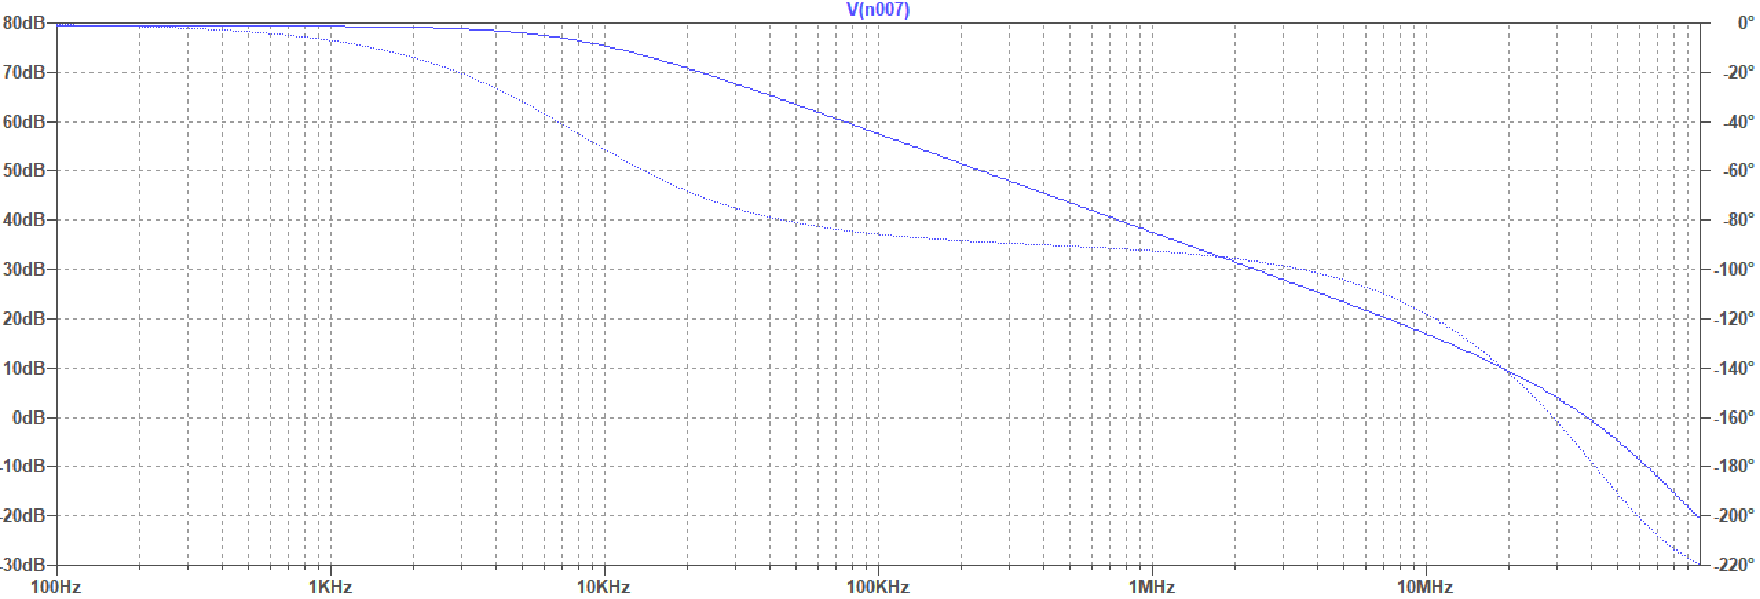
\includegraphics[clip, trim=0 0 0 0, width=1\textwidth]{Sections/7_SystemDesign/Figures/7_1_1_5_DAC_PWR_AMP_150PF.pdf}
    \caption{The simulated open-loop response of the DAC power amplifier with a load  of \SIQ{150}{\pico\farad} and a range resistor of \SIQ{1}{\ohm}.}
    \label{fig_7_1_1_5_DAC_POWER_AMP_SIM_150PF}
\end{figure}

To explain the couse of this instability, the output can be more closely analyzed, under the assumption that the output impedance of the transistors is \SIQ{0}{\ohm} the output $V_o$ is simply a voltage devider betweem $Z_{DUT} + R_{Range} + 2R_o$ and $\frac{Re}{2}$. This simplification can be seen in figure \refq{fig_7_1_1_5_DAC_PWR_AMP_PZ}.

\begin{figure}[H]
    \centering
    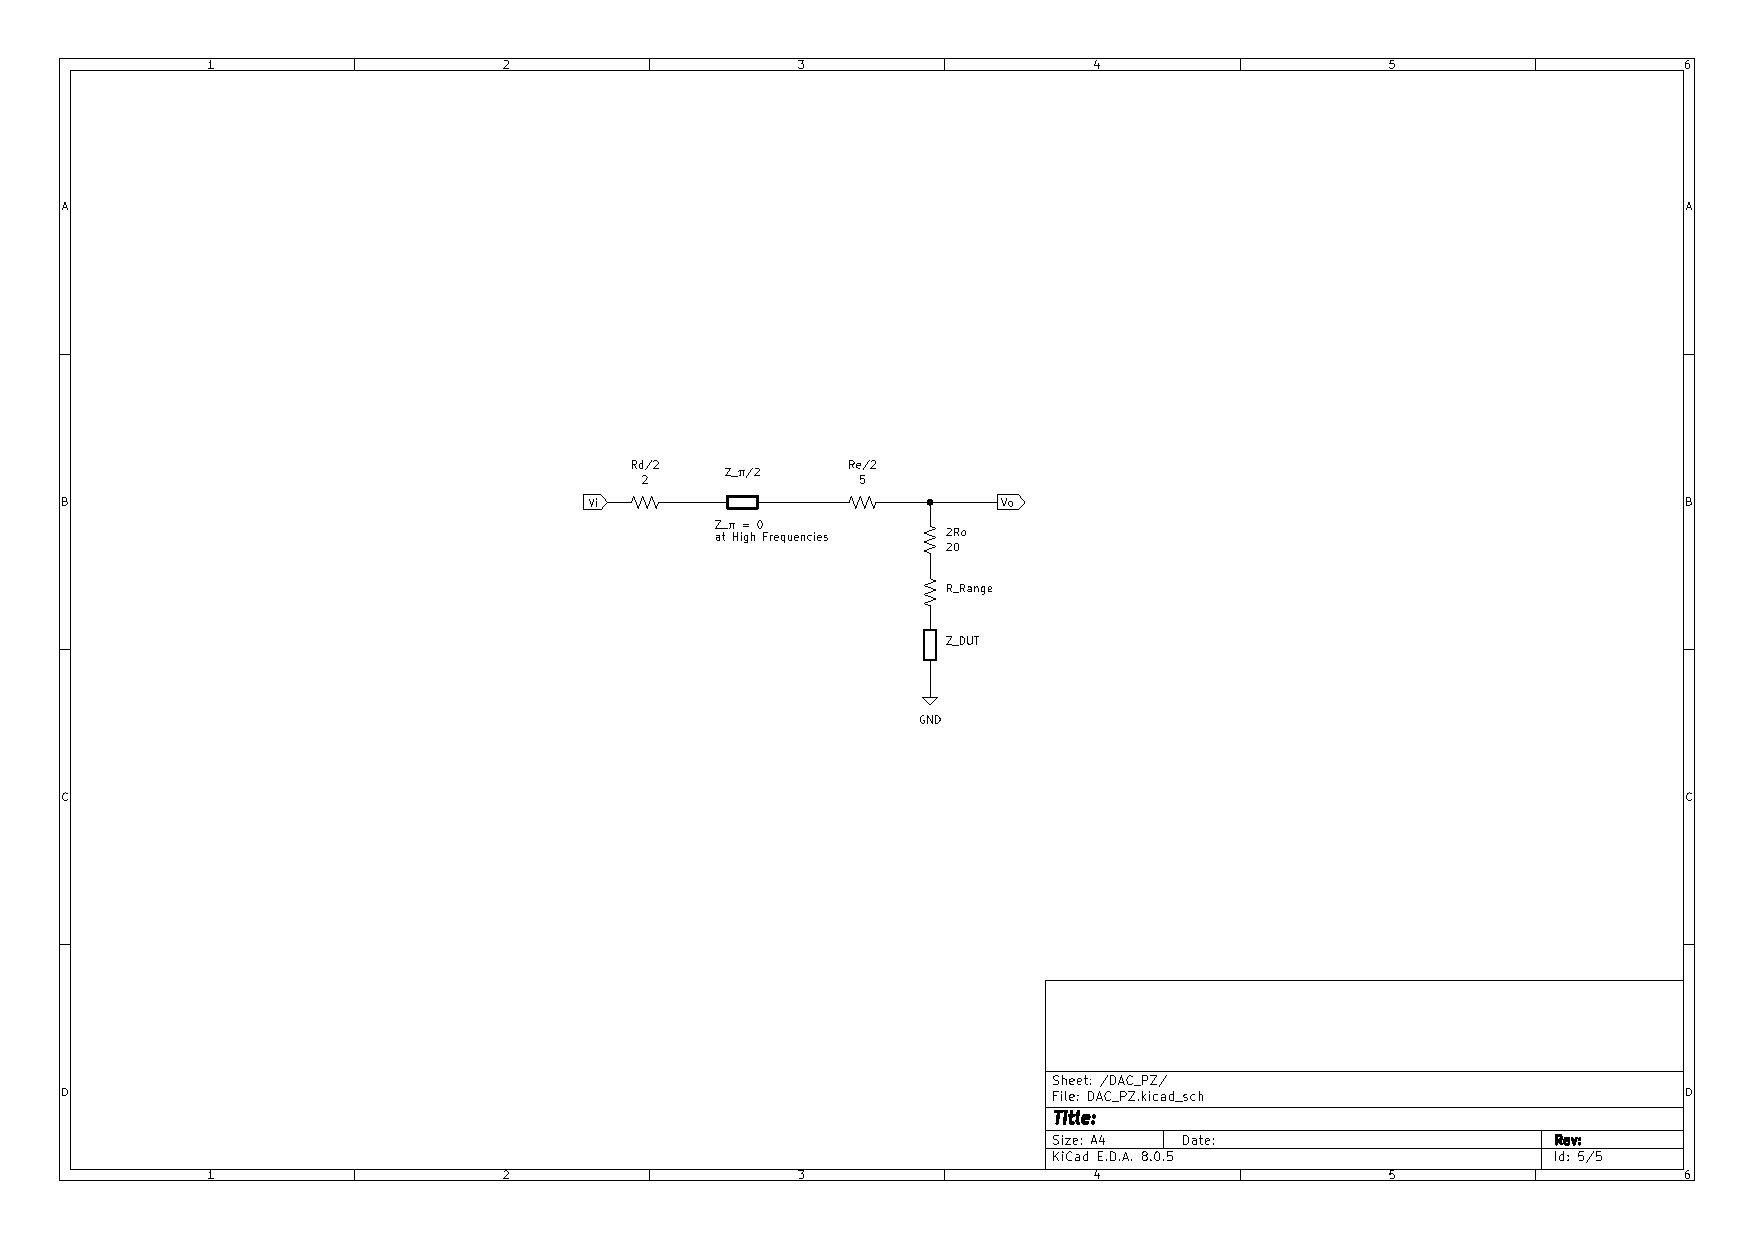
\includegraphics[clip, trim=260 240 280 220, width=1\textwidth]{Sections/7_SystemDesign/Figures/7_1_1_5_DAC_FILTER_DAC_PZ.pdf}
    \caption{Simplified output voltage devider of the power amplifier, $v_i$ is the output of the simplified transistor and $v_o$ is the node that would be feed back into the inverting input of the op-amp in closed loop operation.}
    \label{fig_7_1_1_5_DAC_PWR_AMP_PZ}
\end{figure}

Here $v_o$ can described as a voltage devider

\begin{equation}
\label{eq_DAC_PWR_1}
\begin{split}
    \frac{v_o}{v_i} &= \frac{2R_o+R_{Range}+Z_{DUT}}{2R_o+R_{Range}+Z_{DUT}+\frac{R_e}{2}} \\
    Assuming \:\: &a \:\: capacitive \:\: load. \\
    \frac{v_o}{v_i} &= \frac{2R_o+R_{Range}+\frac{1}{sC}}{2R_o+R_{Range}+\frac{1}{sC}+\frac{R_e}{2}} \\
    \Rightarrow \frac{v_o}{v_i} &= 
\end{split}
\end{equation}